%\documentclass{report}
\documentclass{elsarticle}
%\documentclass{article}
%\documentclass{IEEEtran}


\usepackage[utf8]{inputenc}
\usepackage[a4paper]{geometry}
\usepackage{subfiles}
\usepackage{pdfpages}
\usepackage{multicol}
\usepackage{graphicx}
\usepackage[export]{adjustbox}
\usepackage{float}
\usepackage{booktabs} %make table look good
\usepackage{amsmath}
\usepackage{amssymb}
% \setlength{\parskip}{1.5em}
\graphicspath{./Assets/}

\usepackage{verbatim}

\usepackage[style = ieee]{biblatex}
\addbibresource{./Assets/TestLatex.bib}

\newcommand{\sba}{\sigma_{\beta_a}}
\newcommand{\sbb}{\sigma_{\beta_b}}

\title{LaTeX Workshop 01}
\author{Han Xiong}
\date{25 July 2020}

\begin{document}
\onecolumn
\maketitle
 \tableofcontents
 \listoffigures
 \listoftables
 \newpage
\begin{abstract}

    Lorem ipsum dolor sit amet, consectetuer adipiscing elit. Aenean commodo ligula eget dolor. Aenean massa. Cum sociis natoque penatibus et magnis dis parturient montes, nascetur ridiculus mus. Donec quam felis, ultricies nec, pellentesque eu, pretium quis, sem. Nulla consequat massa quis enim. Donec pede justo, fringilla vel, aliquet nec, vulputate eget, arcu. In enim justo, rhoncus ut, imperdiet a, venenatis vitae, justo. Nullam dictum felis eu pede mollis pretium. Integer tincidunt. Cras dapibus. Vivamus elementum semper nisi. Aenean vulputate eleifend tellus. Aenean leo ligula, porttitor eu, consequat vitae, eleifend ac, enim. Aliquam lorem ante, dapibus in, viverra quis, feugiat a, tellus. Phasellus viverra nulla ut metus varius laoreet. Quisque rutrum. 
    
    
\end{abstract}
%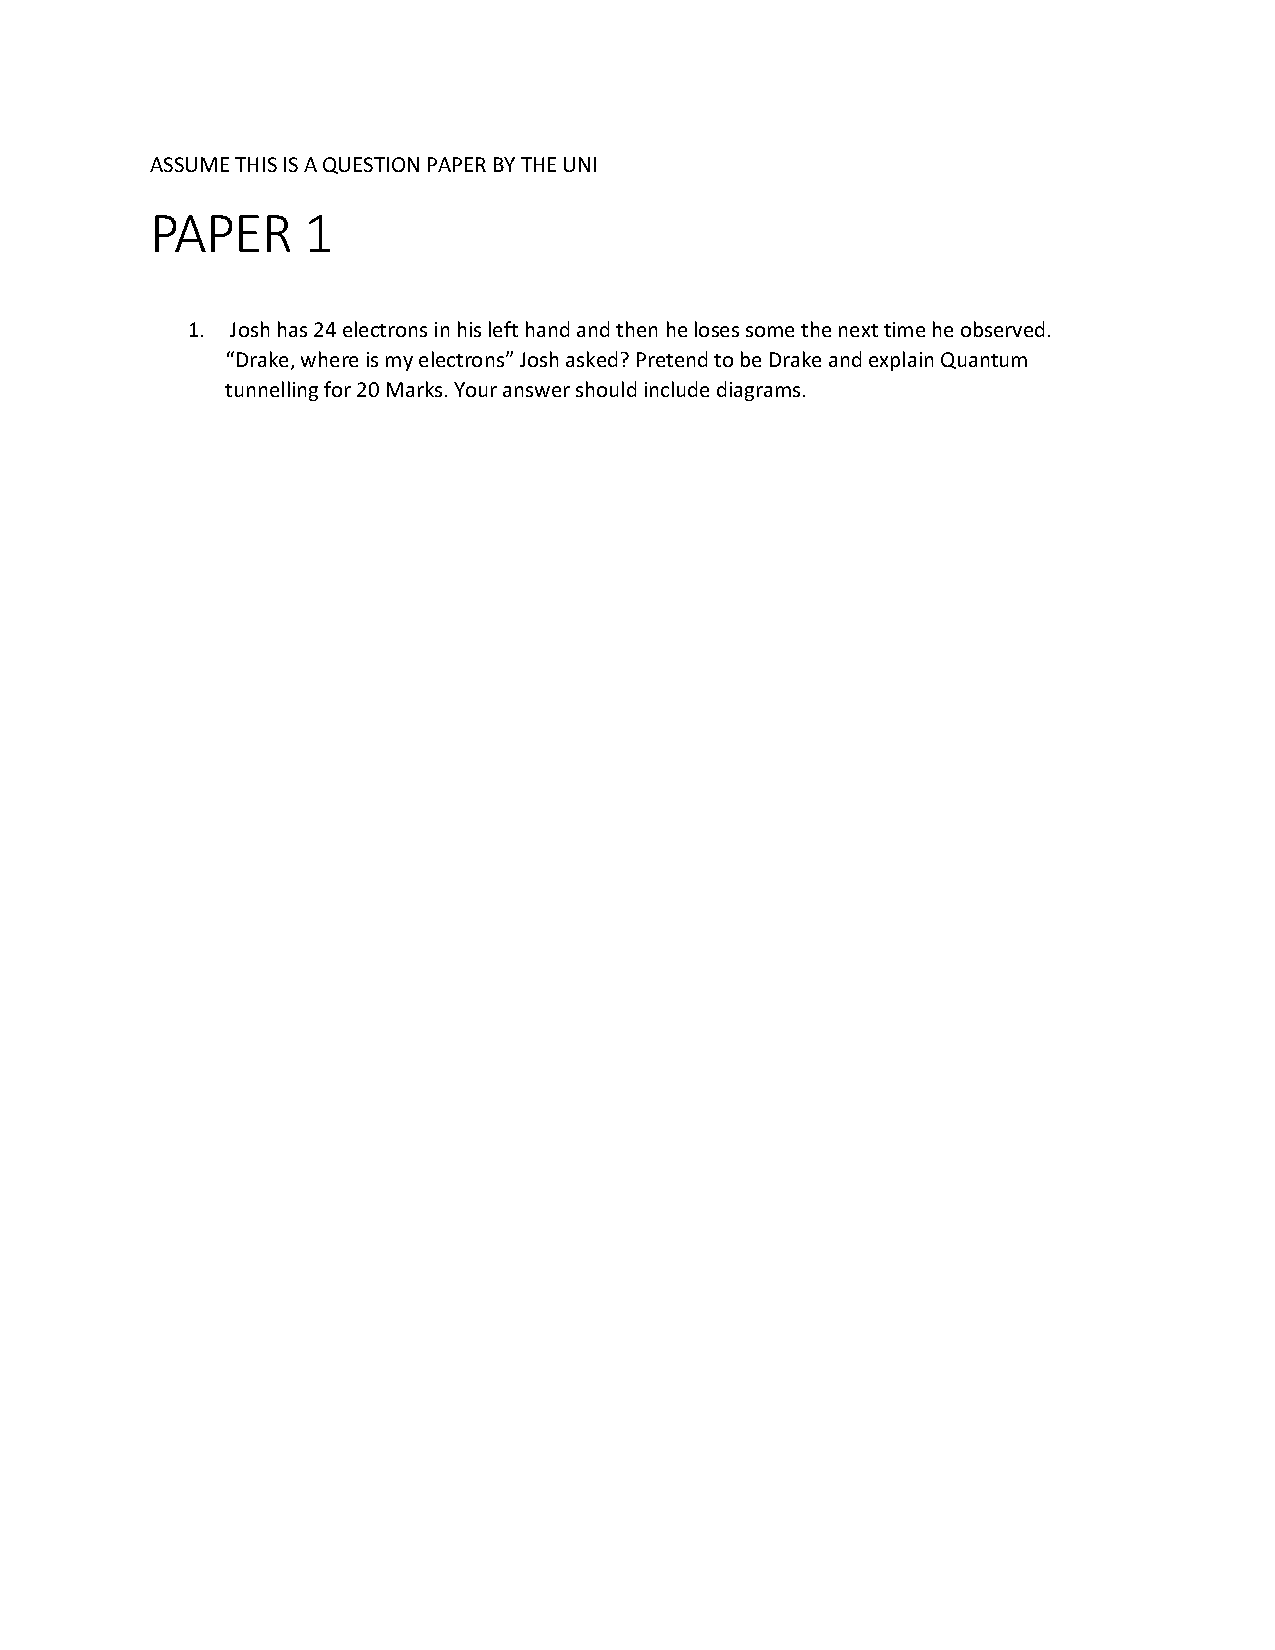
\includepdf[]{./Assets/UNI PAPER}


\subfile{./Methodology/Introduction}
\subfile{./Methodology/Methodology}

\onecolumn

\subfile{./Methodology/Result}

\subfile{./Methodology/Math}

\subsection{Code}
\begin{verbatim}
    Roses are red,
    Violets are blue,
    I miss you too.
    
    from random import randint
def main():
    # Make function work with pandas df afterwards
    name_of_anime = input("Enter Name of Anime:")
    numberEpsSeason1 = input("Enter the number of episodes in Season 1:")
    SlappeNotFound = True 
    Episodes = list(range(0,int(numberEpsSeason1)))

    while(SlappeNotFound and (len(Episodes)>0)):
        sample = int(Episodes.pop(randint(0,len(Episodes)-1)))
        print(f"See if Slappe Present in {sample}")
        prompt = input("Enter Y if slappe found: ")
        if prompt.lower() == 'y':
            SlappeNotFound = False
            print(f"{name_of_anime} Slappe Sample from Episode {sample}")
        if (len(Episodes)==0):
            print("No Slappe Found in this Series - Sample Invalid")

if __name__ == "__main__":
    main()
\end{verbatim}

\verbatiminput{./Assets/randomCode.py}

\section{References}
\subsection{References}
\subsubsection{References}
\printbibliography
\end{document}
